\section{\projectname{} Design} \label{\projectname{}}
Data structure thread-safety in multi-threaded application introduces huge overhead. Efficient design should reduce concurrent access to data structure. In a simple design, we just need a list of pointers to the object. When object is freed, pointers are read from the list and invalidated. This simple design has following issues in multi-threaded environment. $1)$ Multiple threads writing to the same object list need to synchronized (i.e. object to metadata lookup need to be synchronized). $2)$ When pointer is no longer pointing to the same 
object, it should be removed from the list. Pointer to object metadata lookup is used to remove pointer information from the object metadata. Therefore, pointer to object metadata lookup need to be synchronized. $3)$ Same pointer can be inserted multiple times in the object list. \dangnull{} and \freesentry{} maintains pointer-object relationship. Relationship information does not change when pointer keeps pointing to the same earlier object. When pointer points to a new object, old relationship is removed and new relationship is inserted. Therefore, we need thread synchronization for object to metadata and pointer to metadata access. \\% We need to protect concurrent access when objecct to data structure looku and pointer to object lookup. % We need  

Pointer remains in the old object list even after it no longer points to the object. This can lead to incorrect pointer invalidation when old object is freed. Pointer value can be checked to prevent incorrect pointer invalidation. Pointer is invalidated only when pointer points to any inbound object address. The same technique is needed when pointer is modified in non-instrumented code. We do not need pointer to object metadata. Also, removal of old pointer-object relationship adds extra performance overhead. Therefore, pointer to object lookup can be skipped, thereby removes need for a thread synchronization. Concurrent access to per object metadata (list) cannot be skipped. In a simple design, pointer list per object is required. Pointer list is equivalent to a log of pointers. Now, reducing concurrent access to pointer list per object boils down to a well-known problem of concurrent logs. Mostly, concurrent logging is on per-Thread basis. Concurrent logs are write efficient but with costly reads. \\

Normally, number of pointer propagations are higher than the number of object allocations and deallocations. Therefore, pointer propagation tracking should be efficient. One approach is to  skip pointer-to-object metadata lookup. That is no need to maintain old pointer-object relationship. This operation is equivalent to log-write. Motivated by the fact that log-write is efficient, we designed per-Thread per-object log data structure to track pointers pointing to the object in the log. Log read is required when object is freed. The design is similar to a log-structured file system \cite{rosenblum1991design} that maintains circular buffer to track I/Os. The design rationale behind \projectname{} is that the number of pointer registrations (write) are higher than the number of objects free (reads).

\begin{figure}[t]
\center
  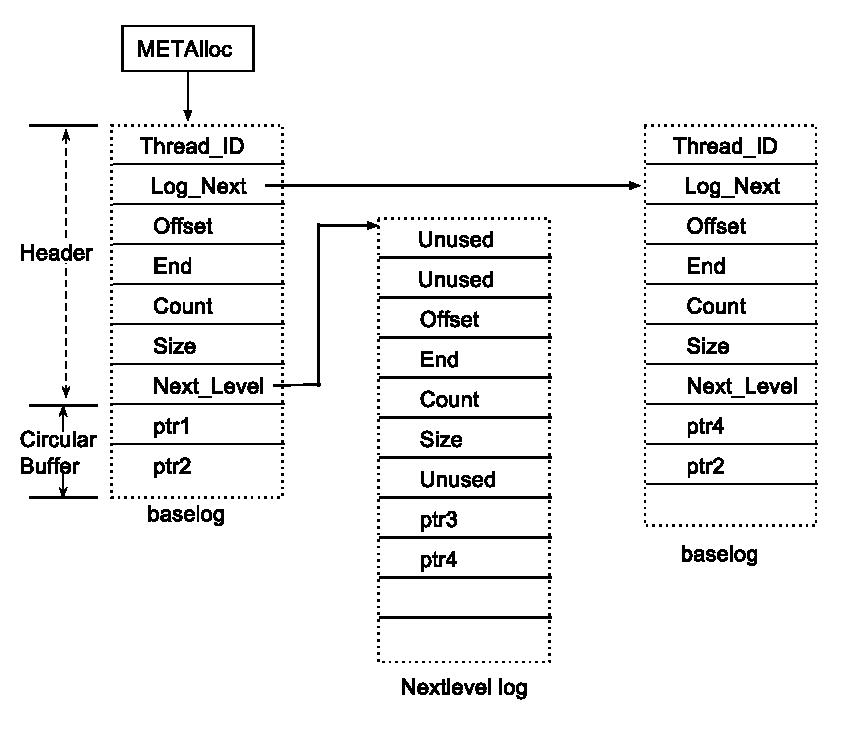
\includegraphics[width=2.8in,height=2.4in,keepaspectratio]{figures/dangsang_design.eps}
  \caption{DangSan data structures for two threaded application.}
  \label{fig:dangsang_design}
  %\vspace*{3in}
  \vspace{-1em}
\end{figure}

\subsection{System Overview}
Figure~\ref{fig:dangsang_design} shows \projectname{} design. Every object metadata has per-thread log. As we are not maintaining pointer-object relationship, only pointer address is needed and stored in the log. Object to metadata lookup retrieves corresponding log for a thread. Pointer tracking function retrieves corresponding log and writes pointer address into it. When object is freed, all per-Thread logs are retrieved. Pointer addresses are read from all the logs and invalidated. During invalidation, current value of pointer is read and checked to see whether it still points to the object. \\  

% Issues: Thread ID, per thread storage
\textbf{per-Thread Storage.} 
We need efficient retrieval of per-Thread log for a given object. One approach is to maintain object lookup table per-Thread. Similar to global shadow memory technique, it should also support range queries. Moreover, maintaining per-Thread object lookup table will incur huge memory overhead. Second approach is shown in Figure~\ref{fig:dangsang_design}, where per-Thread log is maintained in global object list. Maintaining global object list (dynamically) needs thread synchronisation. Another approach is to maintain a static array of log pointers per object. Thread specific \emph{ID} can be used as index into the static array to retrieve corresponding log. Though this approach uses fast array indexing, it has high memory requirements. Second approach is memory efficient but needs concurrent access support. Log removal from dynamic object list is needed only during object free and not during pointer propagation or object allocation. Therefore, only concurrent insertions and reads are needed during pointer propagation. Lock-free insertions and reads can be achieved through compare and swap (\emph{CAS}) atomic instruction~\cite{valois1995lock}. Unique thread IDs can be used to identify thread log. One can use thread IDs assigned by the run-time system or maintain own thread IDs. Maintaining own thread IDs can help in reusing IDs. Reusing thread ID helps in reusing thread log. Dynamic object list can grow large when application has too many short lived threads. Thus, reusing thread log is necessary to reduce list traversal. \\ % explain why only insertion is needed % Mention about per thread storage for each objects metadata. We will need then metadata tracking for perThread. It is not global, which will waste memory.


% Issues: Log Overflow
\textbf{Log Overflow.} 
 In \projectname{}, pointer-object relationship is not maintained. That is, pointer addresses are not removed from old object logs. Depending upon the number of pointers to the object per thread, log overflow has to be handled. One approach is to reallocate log with larger size. But, reallocated log address can be different than the old log address. We need deletion operation to modify dynamic list with this new log address. That is, \emph{CAS} atomic instruction for thread-safety can no longer be used easily. Second approach is to allocate new log for the thread and invalidate old log. Log invalidation is performed simply by setting thread ID maintained in the log to an invalid value. This way, thread can retrieve only a new log using thread ID. However, this approach increases length of dynamic list, thereby increases log retrieval time. Another approach is to introduce second level indirect log. Concurrent access is required for base level logs. Figure~\ref{fig:dangsang_design} shows Second level log. It is activated only when the base level log overflows. After base log overflows, each thread will find base log first and then second level log to store  pointer address. %TODO insted of store pointer address, use register pointer address.
Similar to base log, second level log can overflow. This can be handled easily by reallocating second level log with larger size. This operation does not require thread synchronization.  \\
% No information of pointer-object relationship. Increases pointers per logs. Duplicate pointers.
% Reallocating log is not possible because of deletion operation it involves.

We have introduced few terms in our context $1)$ \textit{Unique pointer:}  Pointer address is stored only once in the log (i.e. Pointer has only one entry in the log). $2)$ \textit{Duplicate pointer:} Pointer address is stored more than once in the log (i.e. Pointer has more than one entry in the log) $3)$ \textit{Stale pointer:} A stored pointer in the log that no longer points to the object. $4)$ \textit{Valid pointer:} A stored pointer in the log that points to the object. Choice of second level data structure also depends on the number of \textit{Unique pointers} and \textit{Duplicate pointers}. Hashtable can be used when \textit{Duplicate} pointers are higher than the \textit{Unique} pointers. But, HashTable introduces huge memory wastage.\\

%TODO use this statement in garbage collection.
%Moreover, Garbage collection of \textit{Stale pointers} is required when it dominates the log. It frees some space from the data structure. Intuitively, on a time scale, old pointers tend to have invalid values than the recent pointer. Hastable cannot track pointer registration history. Thus, Circular log seems the best choice for the stale pointers removal.\\

% N-Lookbehind
\textbf{N-Lookbehind.} 
% Why N-Lookbehind? Duplicates are removed. As we are not keeping pointer-object relationship, we need to removed duplicate pointers from the object log.
One of the reason for log overflow is large number of \textit{Duplicate} pointers. One approach to remove duplicate pointers is to look-behind in the log for a pointer i.e. check pointer address against all stored pointers. Checking entire log for \textit{Duplicate} pointers is a heavy operation. However, we can lookbehind \emph{N} last offsets and skip pointer registration when pointer is within N-Lookbehind offset in the log. Normally, the same pointer is used to iterate over the object memory. This iteration occurs within a short period of time (e.g. in the loop). Depending on the value of $N$, we can eliminate large number of duplicate pointers. In normal scenario, \textit{Unique} pointers are less than or equal to object size. When log size grows larger than object size, \textit{Duplicate} and/or \textit{Stale} pointers are higher than \textit{Unique} pointers. Selection of \emph{N} value is critical in removing \emph{Duplicate} pointers but by considering performance overhead. \\

\begin{figure}[t]
\center
  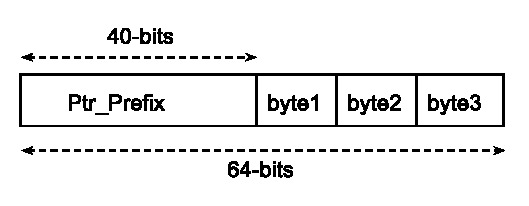
\includegraphics[width=2.8in,height=2.4in,keepaspectratio]{figures/pointer-entry.eps}
  \caption{Pointer entry in the log, where Ptr\_Prefix is a pointer value from 48-bits to 8-bits and byte is a lowermost byte of the pointer}
  \label{fig:pointer_entry}
  %\vspace*{3in}
  \vspace{-1em}
\end{figure}  

Moreover, \emph{N}-Lookbehind can be used to increase log size utilization. On $64$-bit architecture, only lower $48$-bits represent user space virtual memory address. That is, upper most $16$-bits are not used. These two bytes can be used to store two more pointers i.e. (three pointers per log slot). Figure~\ref{fig:pointer_entry} shows a technique to make use of two bytes. We store all three pointers when $40$-bit prefix of all pointers is same. In other word, pointers differing only in lowermost byte can be stored together in the same log slot. Store $40$-bit pointer prefix in the uppermost $40$-bit of the log slot. Next, three remaining lowermost bytes (\textit{byte1}, \textit{byte2}, \textit{byte3}) of the log slot are used to store lowermost byte of three pointers.
Therefore, pointers within $256$ bytes range occupy the same slot in log. Here, \emph{N}-Lookbehind is used to find a log slot where pointer prefix and a log slot prefix match. Following steps can be used to insert pointer into the log, $1)$ Find the empty slot by matching pointer prefix within \emph{N}-Lookbehind entries. Matched slot is empty only when \textit{byte2} or \textit{byte3} is zero ($0x00$). $2)$ When empty slot is found, insert lowermost pointer byte at empty byte location. When pointer lowermost byte is $0x00$, swap this value with $byte1$. That is, pointer byte $0x00$ will always be stored at $byte1$ location. This is because, $0x00$ value denotes empty byte location. $3)$ Skip the registration when \textit{Duplicate} pointer (i.e. both prefix and a byte matched) entry is found. $4)$ When no matching log slot is found, insert $48$ pointer bits into uppermost $48$-bit of new log slot. Thus, \emph{N}-Lookbehind strategy helps in comparing atmost $(N \times 3)$ pointers at the cost of \emph{N} sequential memory access. In best case, log utilization increases by the factor of $3$. \\

% Not sure if we can use this term.????
\textbf{Garbage Collection.} 
Another reason for log overflow is a large number of \textit{Stale} pointers. Normally, with the time, old stored pointers tend to become \textit{Stale}. One approach to remove \textit{Stale} pointers is to treat log as a circular buffer. When log is about to overflow, iterate from log end to \textit{Valid} pointer slot to find \textit{Stale} pointers. Modify log end value with new \textit{Valid} log slot. To determine pointer validity, read pointer value and check whether it still points to the object. For fast check, object bound information can be maintained in the object metadata. We need to grow the log when no \textit{Stale} pointer slot is garbage collected. Note, when we store three pointers per slot, log slot is stale only when all three pointers are stale. Due to garbage collection, amount of work is shifted from object free context to pointer registration context. Total work remains the same with and without garbage collection. Garbage collection avoids log overflow, thereby prevents log reallocation cost. \\

\textbf{Pointer Liveness.} 
\textit{Stale} pointers no longer point to the object. Object in which \textit{Stale} pointer resides may no longer be live (i.e. unmapped). Accessing non-live pointer results into segmentation fault. We access \textit{Stale} pointers in garbage collection and object free routines. To prevent invalid access to \textit{Stale} pointers, one approach is to introduce new action for \texttt{SIGSEGV} signal in garbage collection and object free routines. Ignore \texttt{SIGSEGV} when signal is generated in these routines. Restore old \texttt{SIGSEGV} signal action at the end of above mentioned routines. Another problem with \textit{Stale} pointers is that the pointer memory location might have been allocated to a new object. There exist a small window in object free routine between pointer value check and pointer invalidation operation. In this window, another application thread can write new value to the pointer which may get invalidated wrongly in object free routine. To avoid this problem, we use \emph{CAS} atomic instruction to perform pointer invalidation only when pointer value is old.

\subsection{Static Instrumentation}
Run-time tracking function is instrumented statically using LLVM. Only pointer propagations are tracked (i.e. run-time tracking function is inserted before or after pointer assignment instruction). Allocations (\texttt{malloc}, \texttt{realloc}, \texttt{calloc}, \texttt{new}) and deallocations (\texttt{delete}, \texttt{free}) instructions have to be intercepted if these routines cannot be hooked during run-time. Listing~\ref{lst:staticsrc}\ shows instrumented C code. Run-time tracking function \texttt{track\_ptr()} is inserted after object allocation and pointer propagation code statement (Line $6$ and $8$). \texttt{track\_ptr()} first retrieves metadata for an object and registers pointer address in the metadata. Similarly, \texttt{nullify\_ptr()} is inserted after object deallocation code statement (Line $10$). It retrieves object metadata and invalidates all stored pointer by setting pointer to benign value NULL.    

\lstinputlisting[float, caption=Static Instrumentation, numbers=right, language=C, label={lst:staticsrc}]{Source/static_reg.c} 

We are only interested in pointer assignments.
$$ store\ rhs,\ lhs $$
We track only those store instructions where \textit{rhs} is of pointer type. We pass both \textit{rhs} and \textit{lhs} as arguments to the run-time function. Stack objects are frequently created and destroyed. Benefit of tracking stack object compared to its performance overhead is very low. Similarly, global objects are destroyed (freed) only when application exit. Therefore, we conservatively filter out stores when \textit{rhs} is a stack or global object. Moreover, incorrectly instrumented stack or global objects are skipped during run-time. Also, We skip store instrumentation when $rhs$ is a function pointer or a constant null pointer. When old pointer value is needed in tracking function, insert run-time tracking function before store instruction.  \\

\subsection{Parameters Selection} 
% First discuss what parameters, how it affects performance, solution.
% In the last discuss, emprical results.
Performance of \projectname{} depends on the following three parameters. $1)$ \textbf{N-Lookbehind}: Increasing the value of \emph{N} decreases the number of \textit{Duplicate} pointers. It increases the chance of placing a pointer at already filled log slot. That is, it increases memory utilization of the log. However, increasing the value of \emph{N} introduces cost of reading sequential memory. Distribution of pointer patterns in the log is application specific. Thus, choice of selecting value $N$ depends on the application. $2)$ \textbf{Log Size}: Increasing the log size decreases the number of log reallocations. However, it increases memory wastage. Selection of baselog size (default log size for each thread) and reallocation strategy is critical in maintaining balance between performance overhead and memory wastage. One reallocation strategy is to increase log size additively. This will reduce memory wastage but may need large number of reallocations. Another approach is to increase log size exponentially. This require logarithmic steps to reach maximum needed memory for an object. We perform log resize operation only on the second level log. $3)$ \textbf{Thread-Specific operations}: Thread ID is maintained in thread-specific storage. Also, every log stores thread ID to identify thread-specific log. Maintaining and using thread-specific storage introduces extra memory access and computational checks. These extra performance overhead can be avoided for single threaded applications. One approach is to give compile time option to select the required variant (i.e. single threaded or multi-threaded). Another approach is to maintain thread ID in a register instead of thread-specific storage. Empirically for SPEC2006 benchmarks, $N = 3$ and baselog size $=\ 8$ (number of pointers) with exponential log resize gives better performance.
%TODO Hashtabel approach


%%%% Log size selection

%%%% Talk about the memory that we get for the \projectname{}
%%%% Single-Threaded v/s Multi-Threaded options. Selection of GS/FS register



